\chapter{Modelos específicos de conductores}
\label{ch:specific-models}

En los capítulos anteriores se han decidido los modelos candidatos que conformarán el modelo de comportamiento de conductor general.

Ahora que sabemos cuáles son las técnicas y arquitecturas que mejor se adecuan a este problema con los datos que disponemos, pasaremos a probarlas con los datos de los conductores específicos, comprobando si:

\begin{itemize}
	\item Los errores y precisiones se mantienen en el orden del modelo global.
	\item Los modelos capturan las particularidades de cada sujeto de estudio.
\end{itemize}

Para ello, compararemos primero el modelo longitudinal global con los modelos entrenados de los sujetos. Posteriormente, compararemos los modelos de los sujetos contra los conjuntos de test de cada uno de ellos.

\section{Modelo longitudinal}

La arquitectura que se ha entrenado para cada uno de los sujetos ha sido la $MLP_2$ (topología $7, 8, 4, 1$). En la Figura~\ref{fig:lm-specific-training-validation-and-test-comparison} 

\begin{figure}
	\centering
	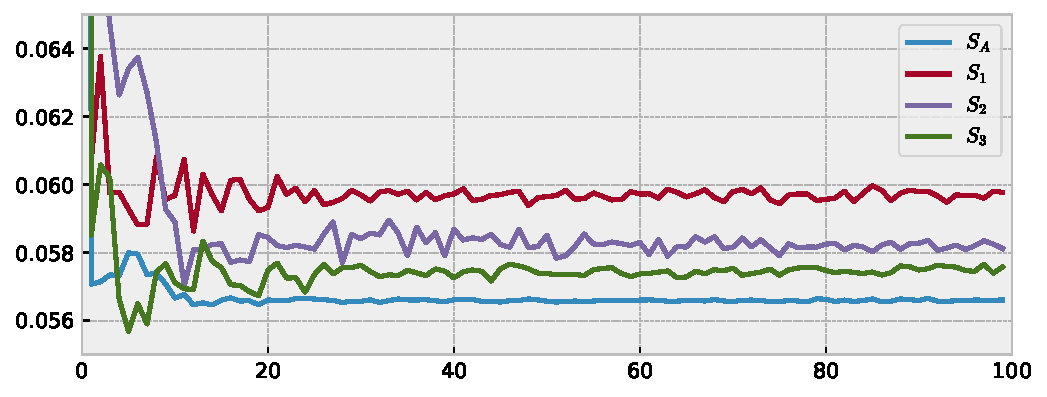
\includegraphics[width=\textwidth]{lm-specific-rmse-all-test-detail}
	\caption[Comparativa de la evolución del error de test entre los sujetos de la arquitectura seleccionada para el modelo longitudinal]{Comparativa de la evolución del error durante el entrenamiento del modelo longitudinal para los sujetos.}
	\label{fig:lm-specific-training-validation-and-test-comparison}
\end{figure}

Se puede observar que el error en test de los sujetos es ligeramente mayor que el del conjunto global. Sin embargo, esto puede ser debido a la mayor capacidad de generalización de éste último al disponer de un conjunto de datos mayor. Los datos del \ac{rmse} se detallan en la tabla~\ref{tbl:lm-specific-rmse}

\begin{table}
	\centering
	\caption[Resumen de los valores de \ac{rmse} para los modelos específicos de comportamiento longitudinal]{Resumen de los valores de \ac{rmse} para los modelos específicos de comportamiento longitudinal.}
	\label{tbl:lm-specific-rmse}
	\begin{tabular}{cccccc}
		\hline
		\multirow{2}{*}{Nombre} & \multicolumn{3}{c}{\ac{rmse}}      \\ 
		& Training & Validation & Test \\ \hline
		$S_A$ & $0.056$ & $0.062$ & $0.057$  \\
		$S_2$ & $0.045$ & $0.039$ & $0.060$  \\
		$S_3$ & $0.039$ & $0.037$ & $0.208$  \\
		$S_4$ & $0.055$ & $0.054$ & $0.058$  \\ \hline
	\end{tabular}
\end{table}

\section{Cambio de carril}

En el caso del modelo de cambio de carril, la arquitectura con la que se han entrenado los modelos específicos es al $CNN_1$ (topología $c16$-$4$-$18$-$v$, $d128$). En la Figura~\ref{fig:lc-specific-rmse-all-test-detail} 

\begin{figure}
	\centering
	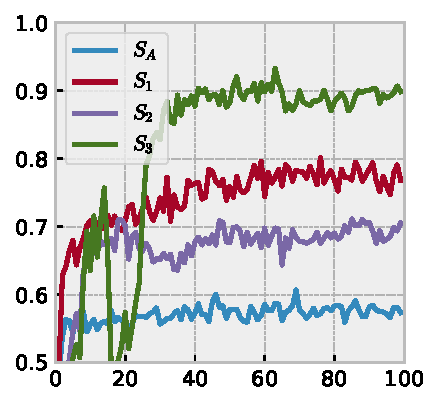
\includegraphics[width=\textwidth]{lc-specific-rmse-all-test-detail}
	\caption[Comparativa de la evolución del error de test entre los sujetos de la arquitectura seleccionada para el modelo de cambio de carril]{Comparativa de la evolución del error de test entre los sujetos de la arquitectura seleccionada para el modelo de cambio de carril.}
	\label{fig:lc-specific-rmse-all-test-detail}
\end{figure}

La precisión alcanzada en los modelos específicos entrenados con esta arquitectura es mayor que la alcanzada por el modelo global. Tiene sentido ya que el modelo global se ha entrenado con el conjunto de datos global y por tanto no obedece exactamente al comportamiento de ningún perfil en concreto, mientras que en los modelos específicos sí. En la tabla~\ref{tbl:lc-specific-accuracy} se exponen los valores de la precisión de este modelo.

\begin{table}
	\centering
	\caption[Resumen de los valores de precisión para los modelos específicos de cambio de carril]{Resumen de los valores de precisión para los modelos específicos de cambio de carril.}
	\label{tbl:lc-specific-accuracy}
	\begin{tabular}{cccccc}
		\hline
		\multirow{2}{*}{Nombre} & \multicolumn{3}{c}{\ac{rmse}}      \\ 
		& Training & Validation & Test \\ \hline
		$S_A$ & $0.056$ & $0.062$ & $0.057$  \\
		$S_2$ & $0.045$ & $0.039$ & $0.060$  \\
		$S_3$ & $0.039$ & $0.037$ & $0.208$  \\
		$S_4$ & $0.056$ & $0.054$ & $0.058$  \\ \hline
	\end{tabular}
\end{table}


\section{Comprobación de personalización de los modelos de conducción específicos}

Las anteriores secciones han mostrado cómo las topologías seleccionadas en los capítulos \nameref{ch:longitudinal-model} y \nameref{ch:lane-change-model} son adecuadas para modelar los comportamientos específicos de cada conductor, además de el conjunto global.

Lo interesante es comprobar si estas topologías son capaces de capturar las diferencias entre conductores. Para ello, comprobaremos cómo se comportan cada uno de los conductores en todos los conjuntos de test.

En el caso del modelo longitudinal, los valores de error cruzados entre sujetos se muestran en la tabla~\ref{tbl:lm-subjects-comparison}.

\begin{table}[]
	\centering
	\caption[Comparación de los errores de aceleración en los diferentes modelos longitudinales]{Comparación de los errores de aceleración en los diferentes modelos longitudinales. }
	\label{tbl:lm-subjects-comparison}
	\begin{tabular}{c|ccc}
		               & \textbf{$S_1$} & \textbf{$S_2$} & \textbf{$S_3$} \\ \hline
		\textbf{$S_1$} & $0.059$        & $0.072$        & $0.070$ \\
		\textbf{$S_2$} & $0.209$        & $0.208$        & $0.213$ \\
		\textbf{$S_3$} & $0.065$        & $0.066$        & $0.057$ \\ \hline
	\end{tabular}
\end{table}

El \ac{rmse} de cada uno de los conductores se mantiene más bajo que el del resto de los sujetos en su propio conjunto de test, aunque no son todo lo bajos que cabría esperar. En la Figura~\ref{fig:lm-subjects-comparison} se muestra gráficamente el perfil de aceleración de cada uno de los conductores sobre cada uno de los perfiles reales.

\begin{figure}[t]
	\centering
	\subfloat[Sujeto $S_1$]{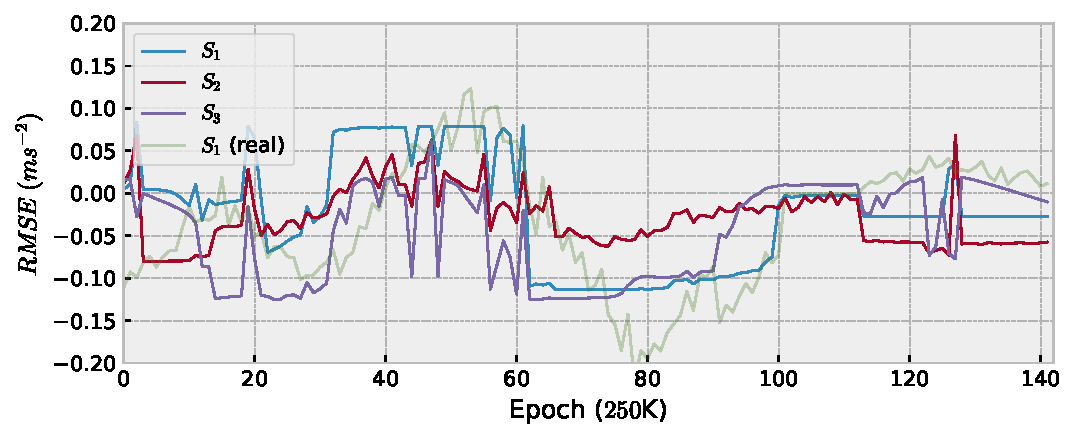
\includegraphics[width=\textwidth]{lm-subjects-comparison-with-edgar-acceleration-profiles}}\qquad
	\subfloat[Sujeto $S_2$]{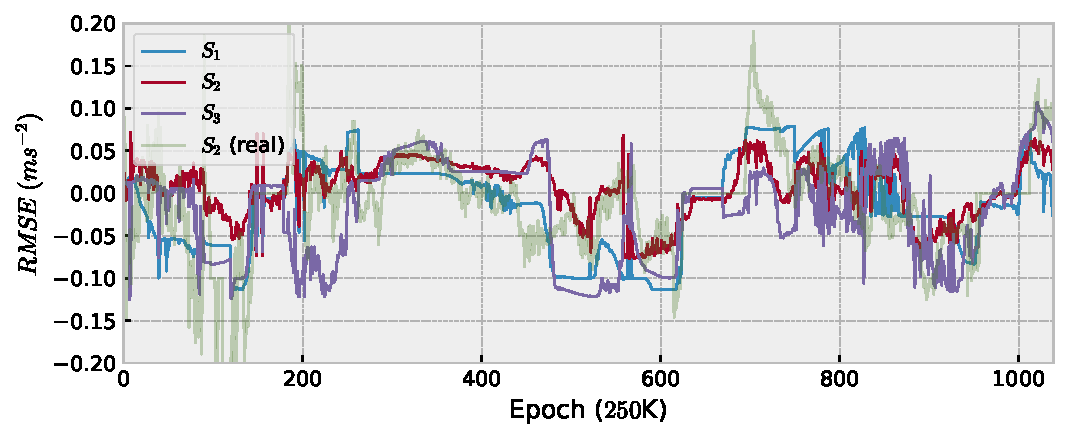
\includegraphics[width=\textwidth]{lm-subjects-comparison-with-jj-acceleration-profiles}}\qquad
	\subfloat[Sujeto $S_3$]{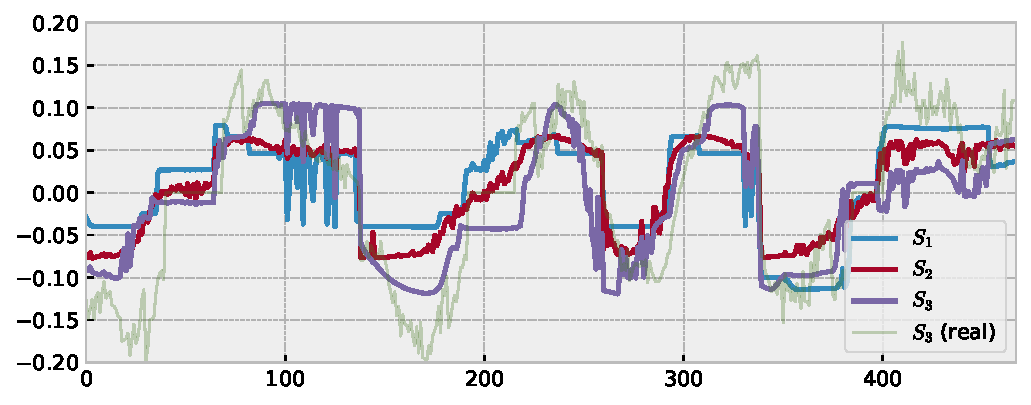
\includegraphics[width=\textwidth]{lm-subjects-comparison-with-miguel-acceleration-profiles}}
	\caption[Perfiles de aceleración de los diferentes sujetos sobre el resto]{Perfiles de aceleración de los diferentes sujetos sobre el resto. Se puede observar que de todos ellos, los perfiles de los sujetos originales se aproximan más a sus respectivos perfiles que los del resto.}
	\label{fig:lm-subjects-comparison}
\end{figure}

En el caso del modelo de cambio de carril, la comparativa la deberíamos hacer con respecto a las tasas de acierto en sus respectivos conjuntos de test. La tabla~\ref{fig:lc-subjects-comparison} muestra los índices de precisión de los sujetos sobre cada uno de los conjntos de test de los demás.

\begin{table}
	\centering
	\caption[Comparación de la precisión para los diferentes modelos de cambio de carril]{Comparación de la precisión para los diferentes modelos de cambio de carril.}
	\label{tbl:lc-subjects-comparison}
	\begin{tabular}{c|ccc}
		& \textbf{$S_1$} & \textbf{$S_2$} & \textbf{$S_3$} \\ \hline
		\textbf{$S_1$} & $0.XXX$ & $0.XXX$ & $0.XXX$ \\
		\textbf{$S_2$} & $0.XXX$ & $0.XXX$ & $0.XXX$ \\
		\textbf{$S_3$} & $0.XXX$ & $0.XXX$ & $0.XXX$ \\ \hline
	\end{tabular}
\end{table}